% Created 2023-01-24 Tue 19:09
% Intended LaTeX compiler: lualatex
\documentclass[11pt]{article}
\usepackage{graphicx}
\usepackage{longtable}
\usepackage{wrapfig}
\usepackage{rotating}
\usepackage[normalem]{ulem}
\usepackage{amsmath}
\usepackage{amssymb}
\usepackage{capt-of}
\usepackage{hyperref}
\usepackage[margin=0.5in]{geometry}
\usepackage{minted}
\author{David Lewis}
\date{1/24/2023}
\title{Lec 5: Classroom activity}
\hypersetup{
 pdfauthor={David Lewis},
 pdftitle={Lec 5: Classroom activity},
 pdfkeywords={},
 pdfsubject={},
 pdfcreator={Emacs 28.2 (Org mode 9.6)}, 
 pdflang={English}}
\begin{document}

\maketitle
\section*{1.}
\label{sec:orgc7abf34}
\begin{itemize}
\item \(\frac{u^Tx}{u^Tu}u = \frac{22}{100}(6, 8) = (1.32, 1.76)\)
\end{itemize}

\begin{minted}[fontsize=\scriptsize]{python}
import matplotlib.pyplot as plt

fig, axes = plt.subplots()

x1 = (0, 1.32)
y1 = (0, 1.76)
x2 = (0, 6)
y2 = (0, 8)
x3 = (0, 1)
y3 = (0, 2)

axes.plot(x1, y1, color="black", linewidth=5)
axes.plot(x2, y2)
axes.plot(x3, y3, markevery=[-1])
fig.savefig("1.png")
\end{minted}

\begin{center}
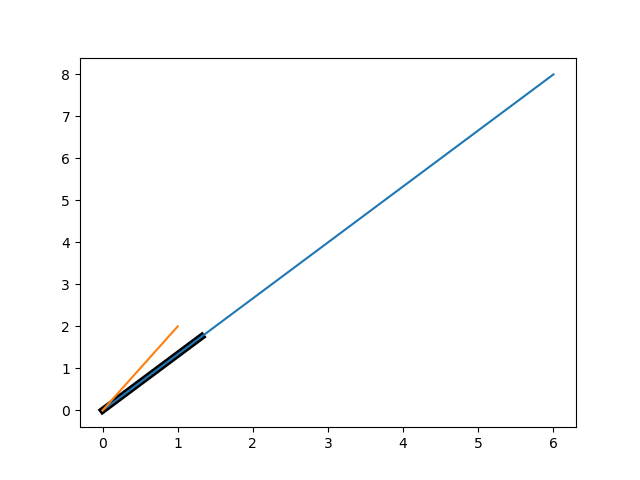
\includegraphics[width=8cm]{1.png}
\end{center}
\section*{2}
\label{sec:org2e2cc01}
\begin{center}
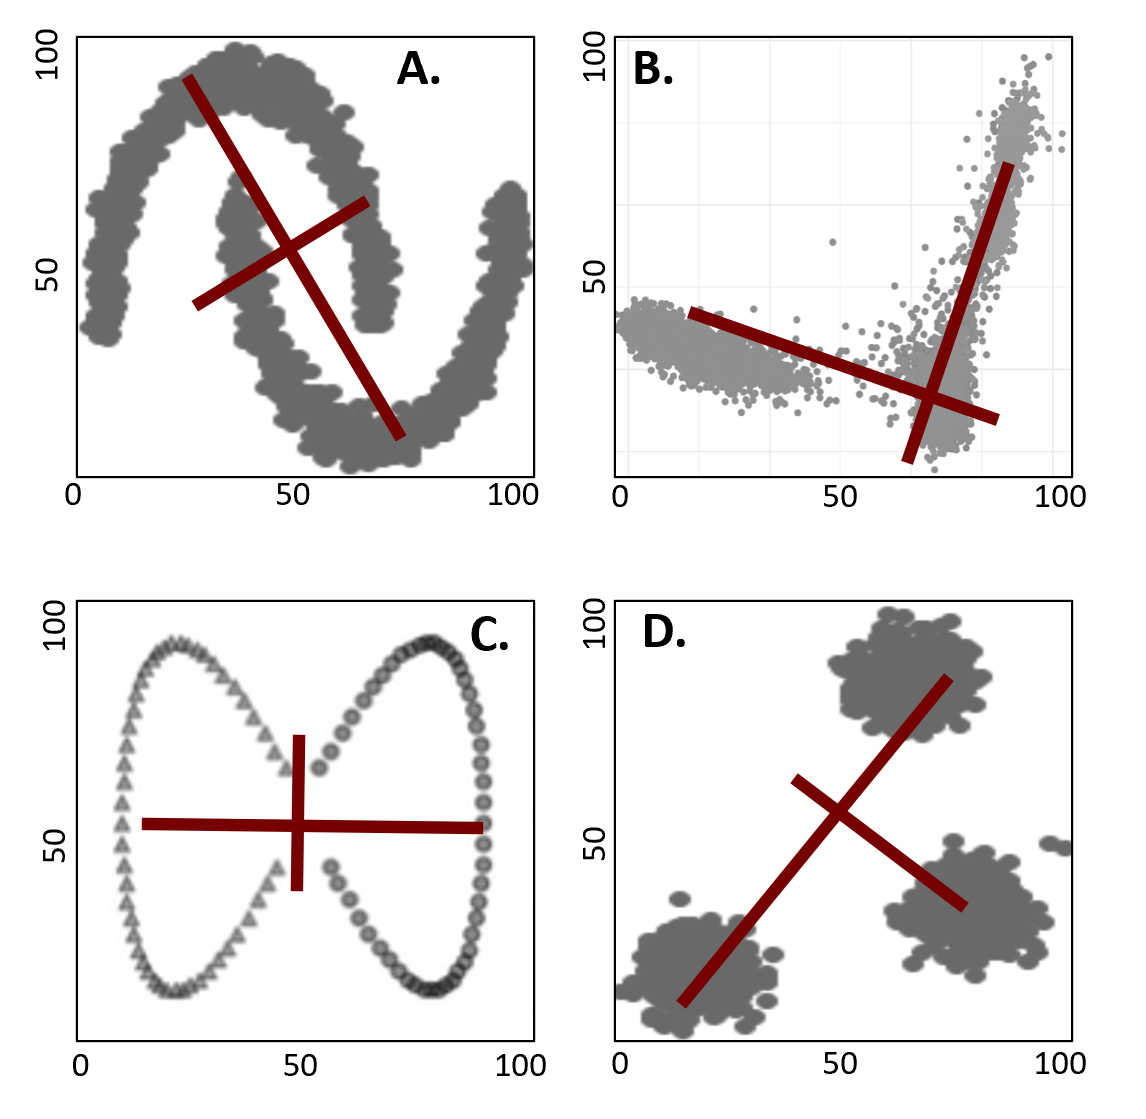
\includegraphics[width=8cm]{2.png}
\end{center}
\begin{itemize}
\item 1 of the plots was roughly parallel to the original axis. This stems from the
fact that 2 dimensions of pca will form an ellipse in 2 dimensions to surround
the data. Most of the data was spread in ways that did not facilitate an
ellipse with parallel axes.
\end{itemize}
\section*{3}
\label{sec:org41fbc1f}
\begin{itemize}
\item \(\sigma_{jk} = \frac{\sum^n_{i=1}(x^j-\mu_x)(x^k-\mu_x)}{n}\) is the covariance for a particular
element in the covariance matrix (known to be true).
\item \(\Sigma = \frac{\sum^n_{i=1}(x_i-\mu)(x_i-\mu)^T}{n} = \frac{\sum^n_{i=1}A_i}{n}\)
\item \(A_i = (x_i-\mu)(x_i-\mu)^T = \begin{bmatrix} x^1_i -\mu&& x^2_i-\mu && ..&& x^d_i -\mu\end{bmatrix}
  \begin{bmatrix} x^1_i-\mu\\ x^2_i -\mu\\ ..\\ x^d_i -\mu\end{bmatrix} =\)
\item \(\begin{bmatrix} (x^1_i-\mu)^2 && ... && (x^1_i-\mu)(x^d_i-\mu) \\... && ... && ... \\ (x^d_i-\mu)(x^1_i-\mu) && ... && (x^d_i-\mu)^2\end{bmatrix}\)
\item This shows that any particular \(a \in A_i\) has the form \(a_{jk} =
  (x^{j}_i-\mu)(x^{k}_i-\mu)\)

\item This is the same as the numerator of the covariance equation before the summation.

\item \(a_{jk} \rightarrow \frac{\sum^n_{i=1}a_{jk}}{n} = \sigma_{jk}\)

\item \(\Sigma = \frac{\sum^n_{i=1}(x_i-\mu)(x_i-\mu)^T}{n} = \frac{\sum^n_{i=1}A_i}{n}
  = \begin{bmatrix} \frac{\sum^n_{i=1}a_{1,1}}{n} && ... &&
  \frac{\sum^n_{i=1}a_{1,k}}{n}  \\... && ... && ... \\ \frac{\sum^n_{i=1}a_{j,1}}{n}
  && ... && \frac{\sum^n_{i=1}a_{jk}}{n}\end{bmatrix} = \begin{bmatrix} \sigma_{1, 1} &&
  ... && \sigma_{1, k} \\ ... && ... && ... \\ \sigma_{j, 1} && ... && \sigma_{j, k}\end{bmatrix}\)

\item Since the summation and division by scalar has the same properties with
matricies as with scalars, both of these operations affect each of the
elements of the matrix as if they were not in the matrix. So since the
summation and division operations are the same in the formula for \(\Sigma\) as
well as \(\sigma_{xy}\) it can be said that the equation for \(\Sigma\) is true.
\end{itemize}


\section*{4}
\label{sec:org4649c20}
\subsection*{a.}
\label{sec:org435096b}
The largest eigenvalue (4.26) is the one that corresponds to the direction of the most
variance. The smallest eigenvalue (0.84) is one that corresponds to the least
variance. This can be intuitively understood because the covariance matrix in
the new basis is the eigenvalues on the diagonal.
\subsection*{b.}
\label{sec:org0189ec4}
\(\begin{bmatrix} 4.26 & 0 & 0 & 0 & 0 & 0 \\
0 & 3.14 & 0 & 0 & 0 & 0 \\
0 & 0 & 2.0 & 0 & 0 & 0 \\
0 & 0 & 0 & 1.92 & 0 & 0 \\
0 & 0 & 0 & 0 & 1.03 & 0 \\
0 & 0 & 0 & 0 & 0 & 0.84 \end{bmatrix}\)

\subsection*{c.}
\label{sec:orged2452a}
The total variance is the sum of the eigenvalues (4.26 + 3.14 + 2.0 + 1.92 +
1.03 + 0.84 = 13.17 ). The total variance does not
change with basis, which is what occurs during the pca and eigenvalue decomposition.

\section*{5.}
\label{sec:orgd6ba9f3}
\begin{itemize}
\item Input: \(D_{n \times k}, \epsilon\)
\item \(\mu_k = \frac{1}{n}\sum^n_{i=1} x_i\) Compute the mean
\item \(Z_{n\times k} = D_{n \times k} - 1 \cdot \mu^T\) Center the data
\item \(\Sigma = \frac{1}{n}(Z^TZ)\)  compute the covariance matrix
\item \(\lambda_k, V_{n \times k} = eig(\Sigma)\) compute eigenvectors, eigenmatrix
\item \(f(r) = \frac{\sum^r_{i=1}\lambda_i}{\sum\lambda_k}\) define fraction of total variance
function, sum of first r eigenvalues in \(\lambda_k\) divided by the sum of all
eigenvalues in \(\lambda_k\)
\item \texttt{r = 1; while f(r) < (1-} \(\epsilon\) \texttt{); r++}; find lowest value of r to meet criteria
\item \texttt{r=r-1}
\item \(U_r = (u_1, u_2 ... , u_r)\) reduced basis
\item \texttt{return} \(D' = \{d'_i | d'_i = U^T_rx_i, \text{for } i = 1, ..., n\}\)
\end{itemize}
\end{document}
